\chapter{Kravspecifikation}

\section{Aktører}

\begin{figure}[h] \centering
\fbox{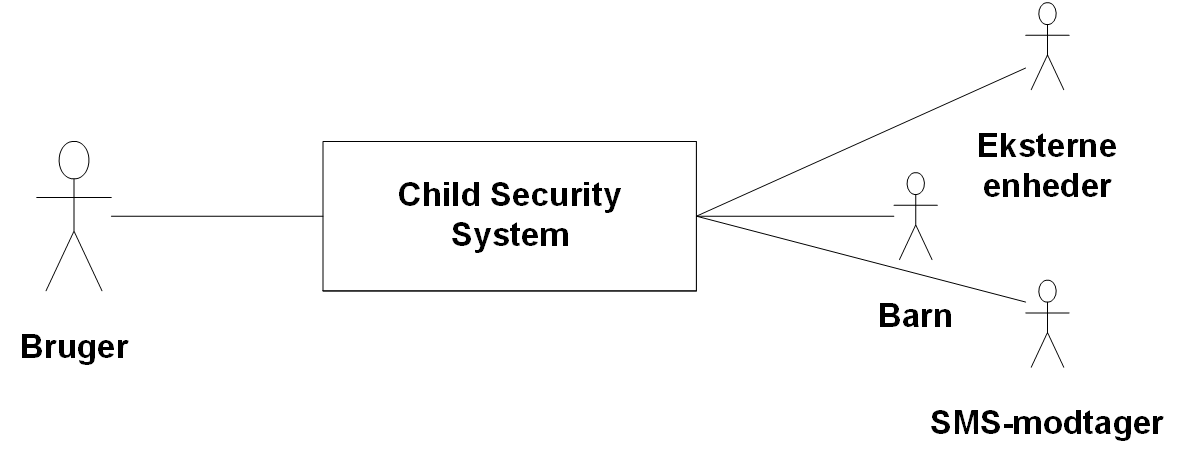
\includegraphics[width=0.6\textwidth]{billeder/Kontekst_Diagram}}
\caption{Kontekst diagram}
\label{lab:kontekstdiagram}
\end{figure}

\subsection{Bruger}
\begin{table}[htbp] \centering
\begin{tabular}{|p{4cm}|p{7cm}|}
	\hline
\textbf{Aktørnavn} &Bruger \\\hline
\textbf{Type Beskrivelse} &
Bruger aktøren er ejeren af systemet eller den voksne med adgang til Computeren.
Dette kunne være, forældre, barnepige osv.	
\\\hline
	\end{tabular}
\end{table}

\subsection{Barn}
\begin{table}[htbp] \centering
\begin{tabular}{|p{4cm}|p{7cm}|}
	\hline
\textbf{Aktørnavn} &Barn \\\hline
\textbf{Type Beskrivelse} &
Barnet eller børnene i huset, som systemet skal beskytte.	
\\\hline
	\end{tabular}
\end{table}

\subsection{SMS Bruger}
\begin{table}[htbp] \centering
\begin{tabular}{|p{4cm}|p{7cm}|}
	\hline
\textbf{Aktørnavn} &SMS Bruger \\\hline
\textbf{Type Beskrivelse} &
Ligesom Bruger (ejeren, forældrene osv.)
Men kan også være naboen eller et familiemedlem der bor i nærheden.
\\\hline
	\end{tabular}
\end{table}

\clearpage		% For at fikse Diagram inde i Section

\section{Usecases}

\begin{figure}[htbp] \centering
\vspace*{\fill}
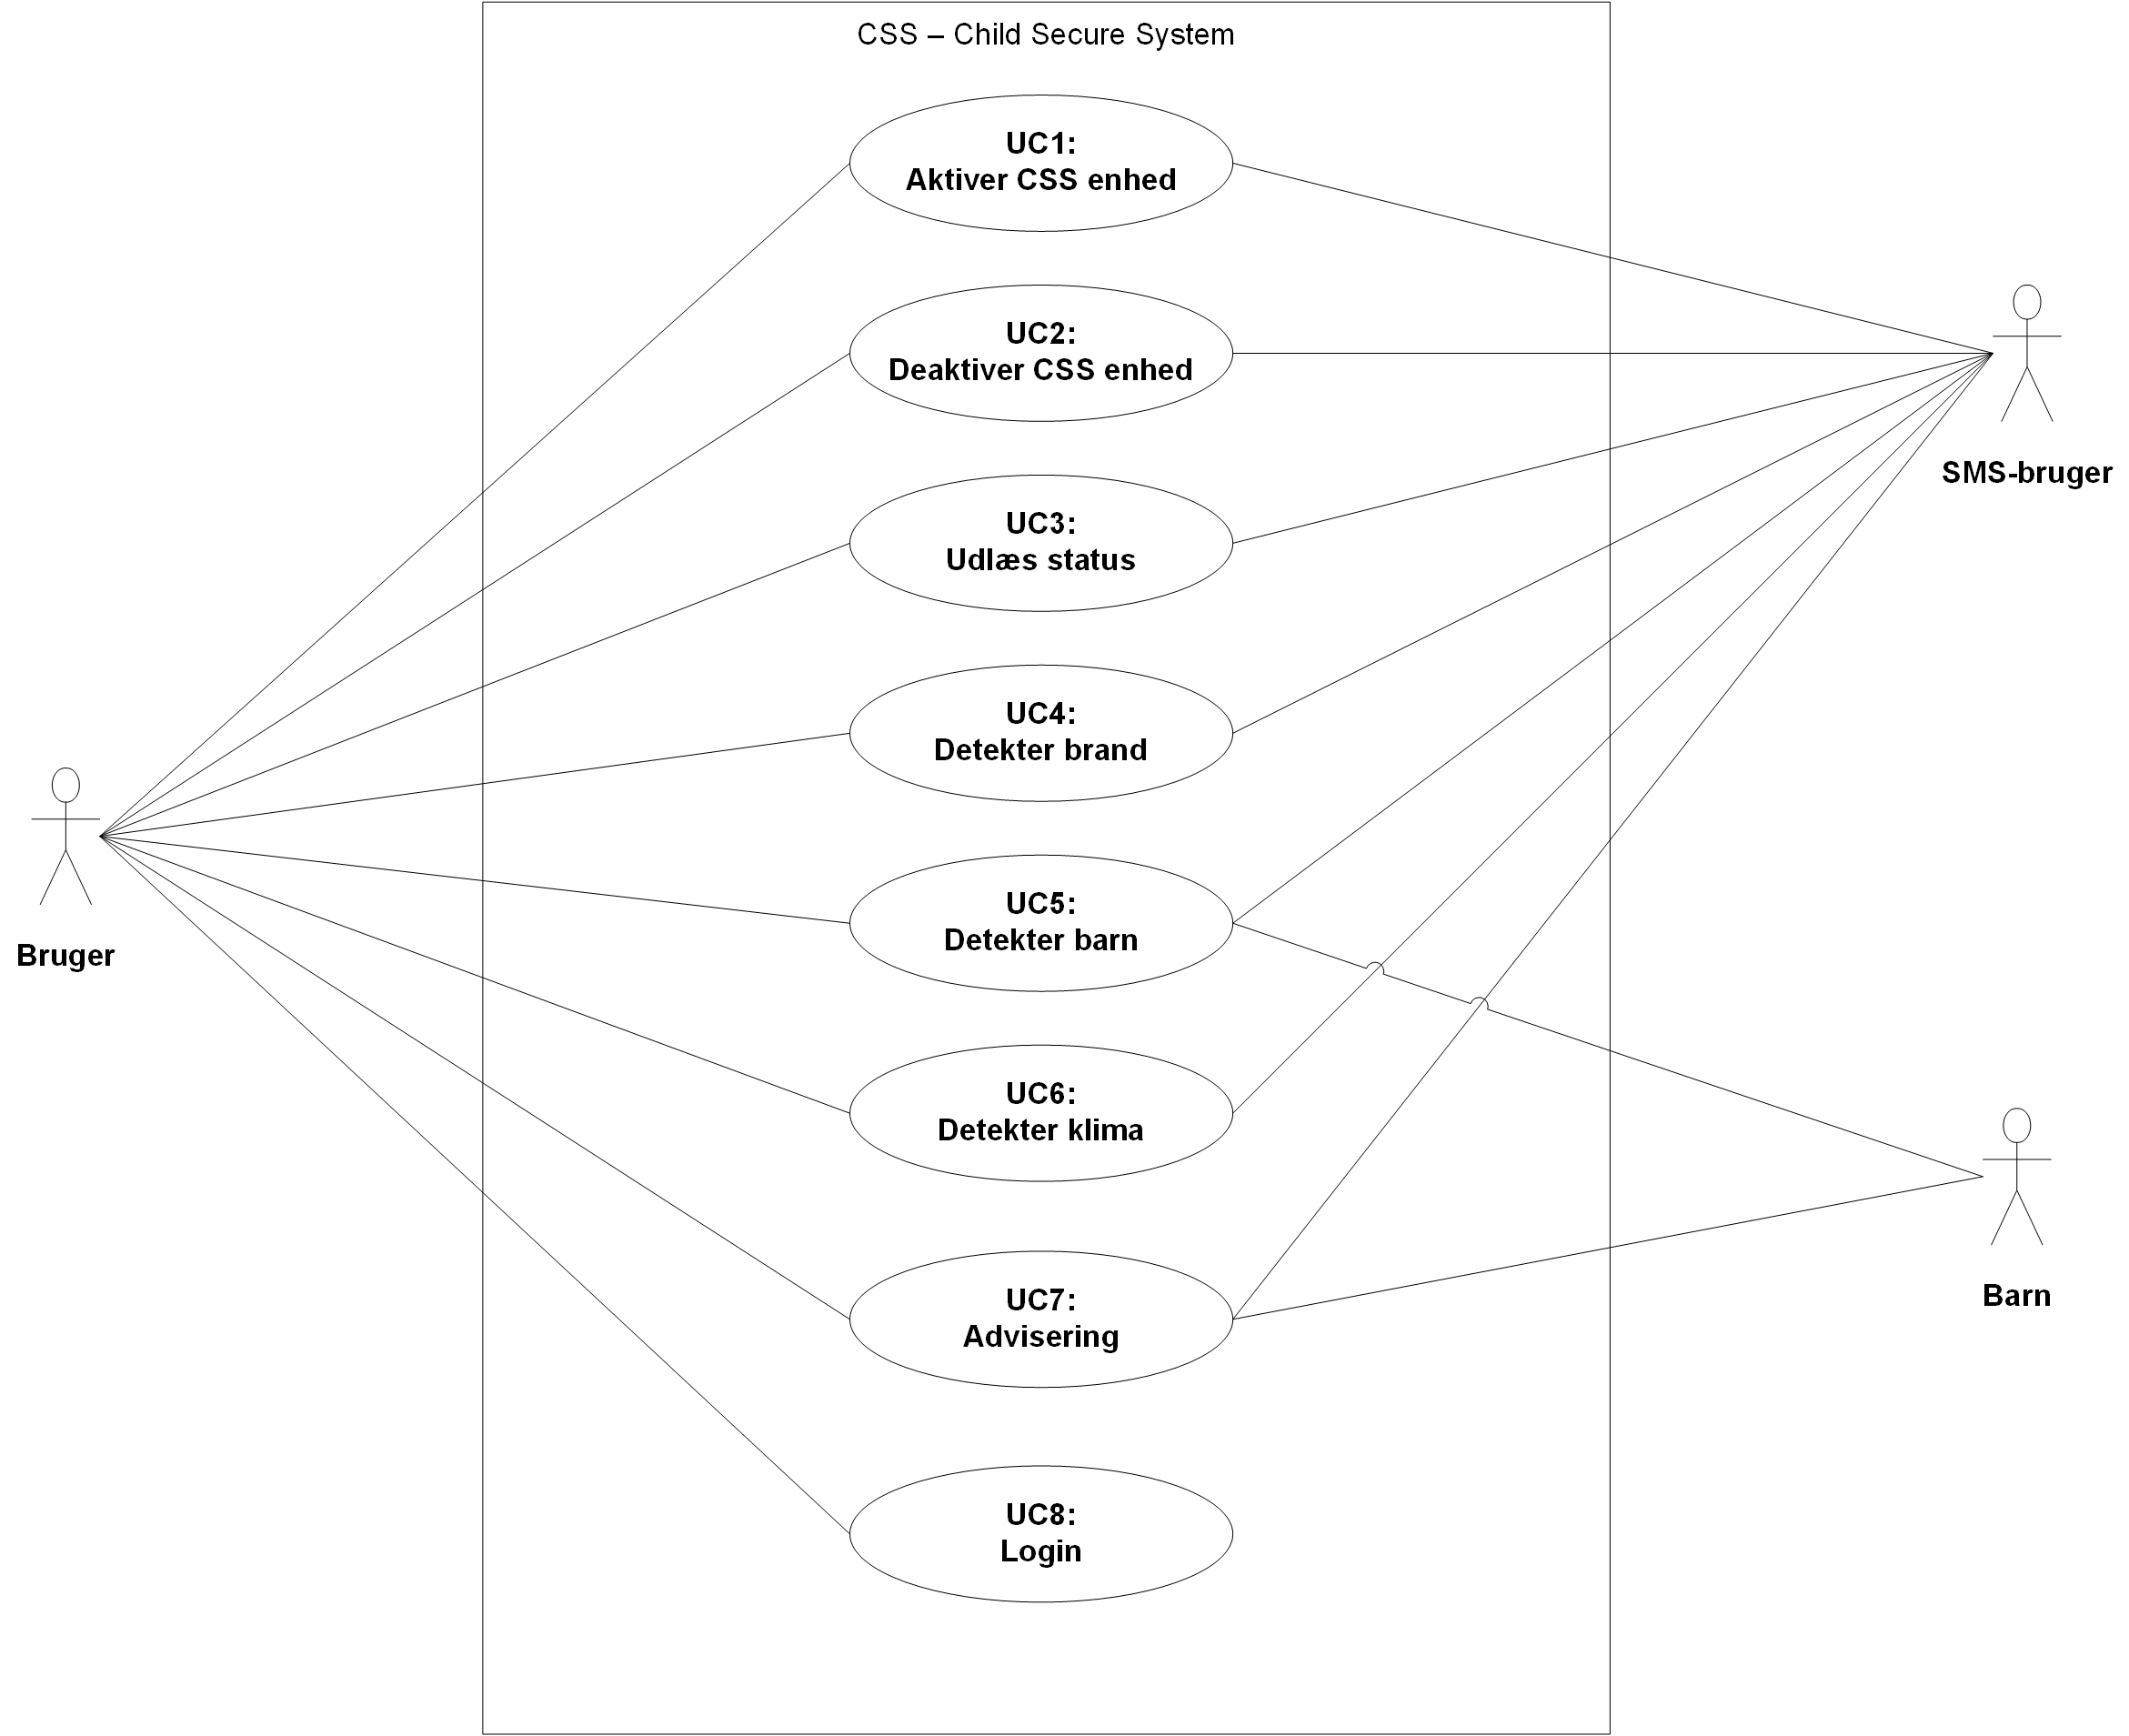
\includegraphics[width=\textwidth]{billeder/Usecase_Diagram}
\caption{Usecase diagram}
\label{lab:usecasediagram}
\vspace*{\fill}
\end{figure}

\subsection{Usecase 1}
\begin{center} \centering
	\begin{longtable}{|p{6cm}|p{8cm}|}
	\hline
		\multicolumn{2}{|l|}{\textbf{UC1: Login}} \\\hline
		\endfirsthead
		
		\multicolumn{2}{l}{...fortsat fra forrige side} \\ \hline 
		\multicolumn{2}{|l|}{\textbf{UC1: Login}} \\\hline
		\endhead		

\textbf{Mål}								
&At Bruger kan logge ind ved hjælp af adgangskode
 \\\hline
\textbf{Initialisering}					
&Bruger vælger login i interface
 \\\hline
\textbf{Aktører og Stakeholders}			
&Bruger(Primær), DE2 Board(Sekundær)
 \\\hline
\textbf{Referencer}						
&Ingen
 \\\hline
\textbf{Antal af samtidige hændelser}	
&1
 \\\hline
\textbf{Forudsætning}					
&At interfacet er tændt
 \\\hline
\textbf{Efterfølgende tilstand}			
&At bruger er logget ind og hovedmenu vises på skærmen. Hele systemet er klar til brug
 \\\hline
\textbf{Hovedforløb}						
& 
\begin{enumerate}

\item Bruger vælger login i interfacet

\item \label{UC2und1}Bruger indtaster 3 koder adskilt af ''Enter'' på DE2 board \newline
\textbf{[Undtagelse \ref{UC2und1}a]} Bruger vælger Annuller

\item Bruger får adgang til hovedmenuen	
 
\end{enumerate}
\\\hline

\textbf{Undtagelser}						
&\begin{enumerate}[label= \ref{UC2und1}a.]
			\item Bruger vælger annuller og kommer tilbage til loginskærm
		\end{enumerate}
\\\hline


		%\textbf{Version}		&1.0 \\\hline
	\end{longtable}
	\label{UC1} 
\end{center}

\subsection{Usecase 2}
\begin{table}[H] \centering
\begin{tabular}{|p{6cm}|p{8cm}|}
	\hline
\multicolumn{2}{|l|}{\textbf{UC2: Deaktiver CSS enhed(er)}} \\\hline
\textbf{Mål}	&
At brugeren kan deaktivere enkelte eller alle enheder, i systemet.
\\\hline
\textbf{Initialisering} &
Bruger trykker "deaktiver", og bliver
præsenteret for hvilke enheder der skal deaktiveres, samt en mulighed for at deaktivere alle
enheder. 
\\\hline
\textbf{Aktører og Stakeholders}	&
Bruger er hovedaktør
\\\hline
\textbf{Referencer} &
Login
\\\hline
\textbf{Antal af samtidige hændelser} &
1
\\\hline
\textbf{Forudsætning} &
At CSS Systemet er helt eller delvist aktiveret.
\\\hline
\textbf{Efterfølgende tilstand} &
Hovedmenu vises
\\\hline
\textbf{Hovedforløb}	&
Bruger trykker deaktiver og følger instruktionerne på skærmen.
\begin{enumerate}
\item Deaktiver alt
\item Deaktiver alle låse
\item Deaktiver babylarm
\end{enumerate}
\\\hline
\textbf{Undtagelser}	&
Ingen
\\\hline
\textbf{Version}		&1.0 \\\hline
	\end{tabular}
	\label{tab:UC2} 
\end{table}

\subsection{Usecase 3}
\begin{table}[H] \centering
	\label{tab:UC3}
\begin{tabular}{|p{6cm}|p{8cm}|}
	\hline
		\textbf{Mål}						&At Bruger kan deaktivere enkelte eller alle enheder, i systemet. \\\hline
		\textbf{Initialisering} 			&Bruger vælger ''Deaktiver'' \\ \hline
		\textbf{Aktører og Stakeholders}	&Bruger(Primær), Eksterne enheder(Sekundær)\\ \hline
		\textbf{Referencer} 				&UC1: Login \\ \hline
		\textbf{Antal af samtidige hændelser} &1 \\ \hline
		\textbf{Forudsætning} 			&Systemet er tændt \\ \hline
		\textbf{Efterfølgende tilstand} 	&Enkelte eller alle enheder er deaktiveret \\ \hline
		\textbf{Hovedforløb}				&

	\begin{enumerate}	
						
					
				\item Bruger vælger ''Deaktiver'' i hovedmenu (UC1 gennemføres)
										
				\item \label{uc3menu}UI viser mulige enheder samt ''Vælg alle'', ''Deaktiver''  og ''Tilbage''
												
				\item Bruger markerer ønskede enheder til deaktivering
												
				\item \label{uc3deact} Bruger vælger ''Deaktiver''\newline
					\textbf{[Undtagelse \ref{uc3deact}a]} Bruger vælger ''Tilbage''
												
				\item \label{uc3sysdeact} Systemet deaktiverer valgte enheder \newline
					\textbf{[Undtagelse \ref{uc3sysdeact}a]} Ingen valgte enheder
				
				\item UI viser besked om at enheder, er deaktiverede
																	
				\item UI returnerer til hovedmenu	
	
	\end{enumerate} \\ \hline

		\textbf{Undtagelser}	
		
		&\begin{enumerate}[label= \ref{uc3deact}a.]
			\item UI returnerer til hovedmenu og UC3 afbrydes
		\end{enumerate}						
							
		\begin{enumerate}[label= \ref{uc3sysdeact}a.]
			\item Hvis ingen enheder er valgt udskrives en fejl på skærmen og beder brugeren om at vælge en enhed og går til UC3.\ref{uc3menu}
		\end{enumerate} \\\hline
											
		%\textbf{Version}		&1.2 \\\hline
		
	\end{tabular} 
\end{table}

\subsection{Usecase 4}
\begin{table}[H] \centering
\begin{tabular}{|p{6cm}|p{8cm}|}
	\hline
\multicolumn{2}{|l|}{\textbf{UC4: Detekter brand}} \\\hline
\textbf{Mål}								&At detektere en opstået brand og eller røgudvikling \\\hline
\textbf{Initialisering}					& CO_2 \\\hline
\textbf{Aktører og Stakeholders}			&Primær: Bruger ønsker at få besked om brand \\\hline
\textbf{Referencer}						& Ingen \\\hline
\textbf{Antal af samtidige hændelser}	& 1 pr. sensor \\\hline
\textbf{Forudsætning}					& CSS sensor aktiv  \\\hline
\textbf{Efterfølgende tilstand}			& Besked til bruger - CSS sensor aktiv \\\hline
\textbf{Hovedforløb}						&  1. CSS sensor aktiv 2. CSS sensor detekterer CO_2  3. CSS sensor udløser alarm (alarm tilstand) 4. Bruger tvinger CSS sensor ud af alarm tilstand\\\hline
\textbf{Tilføjelser}						& Det er muligt at teste sensoren ved at trykke på en knap og herved "illustrere" en brand  \\\hline
%\textbf{Datavariationsliste}			&Test \\\hline
	\end{tabular}
	\label{UC4} 
\end{table}

\subsection{Usecase 5}
\begin{table}[H] \centering
\begin{tabular}{|p{6cm}|p{8cm}|}
	\hline
\multicolumn{2}{|l|}{\textbf{UC5: Detekter barn}} \\\hline
\textbf{Mål}								&At detektere om barnet bevæger sig eller græder \\\hline
\textbf{Initialisering}					&Barnet bevæger sig eller græder\\\hline
\textbf{Aktører og Stakeholders}			&Bruger(Primær): Ønsker at kunne overvåge barnet. SMS Bruger(Sekundær): 																	Modtager SMS ved gråd eller bevægelser. Barn(Sekundær): Ønskes overvåget 				 \\\hline
\textbf{Referencer}						&Advisering \\\hline
\textbf{Antal af samtidige hændelser}	&1 \\\hline
\textbf{Forudsætning}					&At CSS er aktiveret \\\hline
\textbf{Efterfølgende tilstand}			&Sensor stadig aktiv \\\hline
\textbf{Hovedforløb}						&\begin{enumerate}
	
				\item Systemet er aktiveret
												
				\item Systemet opfanger bevægelse eller gråd
												
				\item Systemet kalder advisering
								
			\end{enumerate}\\\hline1.
\textbf{Tilføjelser}					&Ingen \\\hline
%\textbf{Datavariationsliste}			&Test \\\hline
	\end{tabular}
	\label{UC5} 
\end{table}

\subsection{Usecase 6}
\begin{table}[H] \centering
\begin{tabular}{|p{6cm}|p{8cm}|}
	\hline
\textbf{Mål} &
Skriv her  \\\hline

\textbf{Initialisering} &
Skriv her  \\\hline
 
\textbf{Aktører og Stakeholders} &
Skriv her  \\\hline

\textbf{Referencer} &
Skriv her  \\\hline

\textbf{Antal af samtidige hændelser} &
Skriv her  \\\hline

\textbf{Forudsætning} &
Skriv her  \\\hline

\textbf{Efterfølgende tilstand} &
Skriv her  \\\hline

\textbf{Hovedforløb} &
\begin{enumerate}

\item Punkt
\item Punkt

\end{enumerate}   
 \\\hline
 
\textbf{Undtagelser} &Ingen \\\hline
		\textbf{Version}		&1.0 \\\hline
	\end{tabular}
	\label{UC6} 
\end{table}

\subsection{Usecase 7}
\begin{table}[H] \centering
\begin{tabular}{|p{6cm}|p{8cm}|}
	\hline
\textbf{Mål} &
Skriv her  \\\hline

\textbf{Initialisering} &
Skriv her  \\\hline
 
\textbf{Aktører og Stakeholders} &
Skriv her  \\\hline

\textbf{Referencer} &
Skriv her  \\\hline

\textbf{Antal af samtidige hændelser} &
Skriv her  \\\hline

\textbf{Forudsætning} &
Skriv her  \\\hline

\textbf{Efterfølgende tilstand} &
Skriv her  \\\hline

\textbf{Hovedforløb} &
\begin{enumerate}

\item Punkt
\item Punkt

\end{enumerate}   
 \\\hline
 
\textbf{Undtagelser} &
Ingen \\\hline

		\textbf{Version}		&1.0 \\\hline
	\end{tabular}
	\label{UC7} 
\end{table}

% Advisering

\subsection{Usecase 8}
\begin{table}[H] \centering
\begin{tabular}{|p{6cm}|p{8cm}|}
	\hline
\multicolumn{2}{|l|}{\textbf{UC8: Login}} \\\hline
\textbf{Mål}								
&At tilmeldt bruger af systemet kan logge ind ved brug af personlig brugernavn og password
 \\\hline
\textbf{Initialisering}					
&Bruger vælger login i interface
 \\\hline
\textbf{Aktører og Stakeholders}			
&Primær: Bruger
 \\\hline
\textbf{Referencer}						
&Ingen
 \\\hline
\textbf{Antal af samtidige hændelser}	
&Der kan fortages ét login ad gangen (sådan skal det formuleres!)
 \\\hline
\textbf{Forudsætning}					
&At interface er online
 \\\hline
\textbf{Efterfølgende tilstand}			
&At bruger er logget ind og hovedmenu vises på skærmen. Hele systmet er klar til brug
 \\\hline
\textbf{Hovedforløb}						
& 
\begin{enumerate}

\item Bruger vælger login i interface

\item Bruger indtaster personlig brugernavn og adgangskode

\item Systemet validerer brugernavn og adgangskode (Extension 1: Ikke valideret)

\item Bruger får adgang til hovedmenu
 
\end{enumerate}
\\\hline

\textbf{Tilføjelser}						&
ingen \\\hline
%\textbf{Datavariationsliste}			&Test \\\hline
	\end{tabular}
	\label{UC8} 
\end{table}

\subsection{Usecase 9}
\begin{table}[H] \centering
\begin{tabular}{|p{6cm}|p{8cm}|}
	\hline
\multicolumn{2}{|l|}{\textbf{UC8: Login}} \\\hline
\textbf{Mål}								
&At tilmeldt bruger af systemet kan logge ind ved brug af personlig brugernavn og password
 \\\hline
\textbf{Initialisering}					
&Bruger vælger login i interface
 \\\hline
\textbf{Aktører og Stakeholders}			
&Primær: Bruger
 \\\hline
\textbf{Referencer}						
&Ingen
 \\\hline
\textbf{Antal af samtidige hændelser}	
&Der kan fortages ét login ad gangen (sådan skal det formuleres!)
 \\\hline
\textbf{Forudsætning}					
&At interface er online
 \\\hline
\textbf{Efterfølgende tilstand}			
&At bruger er logget ind og hovedmenu vises på skærmen. Hele systmet er klar til brug
 \\\hline
\textbf{Hovedforløb}						
& 
\begin{enumerate}

\item Bruger vælger login i interface

\item Bruger indtaster personlig brugernavn og adgangskode [Extension 1: Bruger vælger Annuller]

\item Systemet validerer brugernavn og adgangskode [Extension 2: Ikke valideret]

\item Bruger får adgang til hovedmenu
 
\end{enumerate}
\\\hline

\textbf{Tilføjelser}						&

Extension 1:

Bruger vælger annuller og kommer tilbage til startskærm

Extension 2: 

Brugernavn eller adgangskode ikke indtastet korret. Brugernavn og adganskode indtastes igen. \\\hline
%\textbf{Datavariationsliste}			&Test \\\hline
	\end{tabular}
	\label{UC9} 
\end{table}
